\subsection{Model explanation}
\textcolor{red}{Add a short introduction to introduce the subsections}
\subsection{How is System Dynamics used?}
An important aspect to system dynamics models are the aforementioned accumulations, delays and feed-backs. Accumulations, more commonly referred to as stock variables refer to some value material or entities within a system. Through flow or rate variables stocks dynamically change over time, leading to the aforementioned delay and feed-back effects \parencite{sterman_system_2001}. To build the sub-models for the study on \textit{Campylobacter} appropriate variables had to be chosen to represent these features. In the case of, infected populations of humans and flocks would act modelled as stocks, whilst various transmission routes provide flow variables between them. This naturally produces delays, as it takes time for the disease to spread, symptoms to surface and potential hospitalisation. Feed-back loops will also arise as \textit{Campylobacter}, as the number of contaminated chicken flocks, causes more spread of \textit{Campylobacter} in the environment, and in turn the more \textit{Campylobacter} in the environment, the more easily chicken flocks are infected. Furthermore the model was subdivided into multiple subsystems, which will be explained in the following paragraphs. 

%1.	Explain basics of SD
 %   a.	Basics of SD
  %  b.	Examples from literature to clarify and justify modelling choices given problem in the field
%2.	Conceptualisation
  %  a.	Depict aggregate model structure
   % b.	Describe dynamic hypothesis

\subsection{Conceptualisation}
\label{s:conceptualisation}
The model will focus on the economic impacts and health care costs associated with \textit{Campylobacter}-contaminated chicken meat. The dynamic hypothesis includes three KPIs that will be examined to answer the research question: 
\begin{itemize}
    % \item Number of infected chicken flocks: is expected to increase with worsening climate conditions and no interventions.
    \item Concentration of \textit{Campylobacter} in surface waters: as climate effects continue on their current trends, \textit{Campylobacter} will be able to proliferate more easily and consequently contaminate more poultry meat. These contaminations would follow an S-growth curve in the coming years considering both a reinforcing loop of the number of contaminated chicken flocks, causing more spread of \textit{Campylobacter} in the environment, and in turn the more campylobacter in the environment, the more easily chicken flocks are infected, but also a balancing loop as surface waters will reach a certain carrying capacity. %too long a sentence?
    \item Amount of environmental transmissions via disease vectors: the prior KPIs would consequently mean that these would also increase drastically, as most transmission routes are likely to display interaction effects.
    % \item Number of infected people: is expected to increase exponentially as reinforcing loops between farms and environment would greatly increase chance of infection but with a less exponential rate than that of infected flock, as different existing hygiene measures exist to reduce/minimise contamination of meat products.
    \item Cost of illness (based on DALY): is expected to increase with increasing \textit{Campylobacter} infection rates, and decrease (at different rates) with the introduction of different policies.
\end{itemize}
 
\begin{figure}[h]
\centering
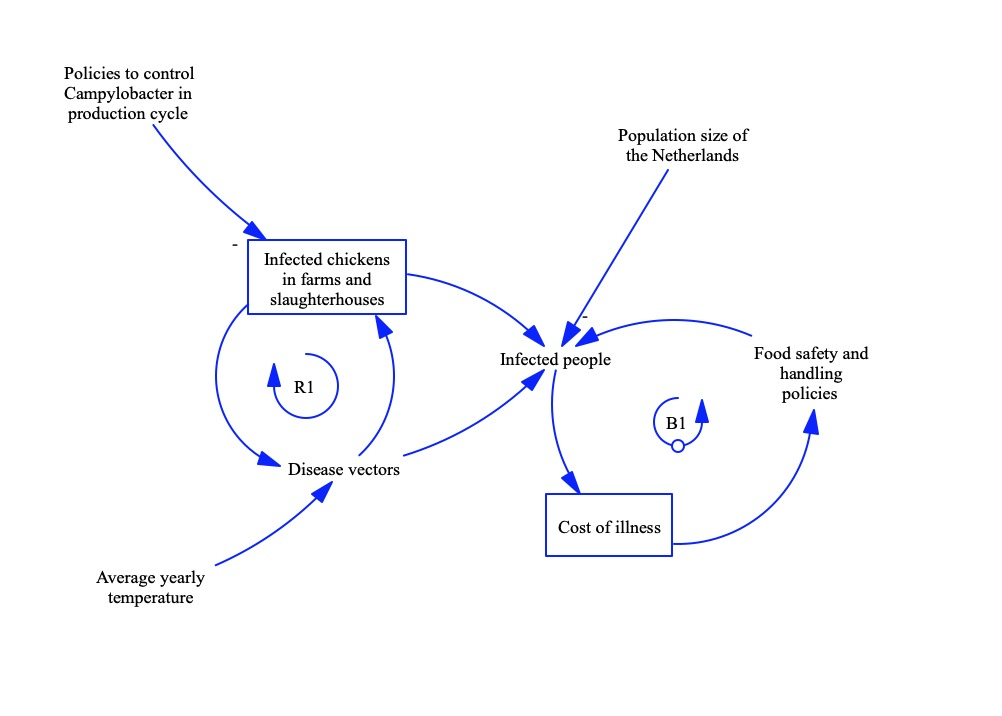
\includegraphics[width=\textwidth]{images/dynamic_hypo.jpeg}
%0.5 text width is too small man
\caption{The aggregated causal loop diagram for the dynamic hypothesis}
\end{figure}
 
\subsubsection*{Model Structure}
Although contamination is mainly concentrated on farms, the model will focus on farms and slaughterhouses collectively, rather than individual types of farms. This aligns better with decision-making regarding the general impacts of policy choices across the entire poultry industry in the Netherlands. This level of aggregation excludes most of the internal processes of slaughterhouses and broilers, as these are too detailed for this scope. Furthermore, this model will be tested against several climate scenarios which are based on the following assumptions: no new insect species are introduced into the system, despite their connection to climate change effects and spread of \textit{Campylobacter}, their influences were considered too detailed relative to the problem scoping. Lastly, the human population will be split into cohorts of children, working-age and seniors. Although cohorts based on age ranges would provide more accurate representation, the DALY used to calculate this cost of illness already incorporates age weightings \parencite{mangen_campylobacteriosis_2007}. 
\subsubsection*{Model Boundaries}

This model draws wider boundaries than Rommens' original model \parencite{rommens_infected_2020}. Here, the focus is on climate, population, and policy effects (both on production and consumption) and the subsequent economic impacts of these factors. As a result, some internal components of the model were simplified. Specifically, operational components related to transmissions occurring on individual farms, broilers, and slaughterhouses were aggregated into a single sub-model, allowing for more focus on environmental transmission pathways.

The sub-model of 'Infected Chickens' encompasses the majority of Rommens' original model \parencite{rommens_infected_2020}. Details of the structure and behaviour of this sub-model are detailed in the following sections.

\subsubsection*{Dynamic Hypothesis}
% is it okay to merge with conceptualisation?
% yes, I think so - M

\subsection{Explanation of model}
%3.	Explain model (also refer to Appendix A)
 %   a.	Describe sub-models
  %  b.	Explain most important assumptions
   
This analysis contains three main sub-models:

%Z: shorten the list in a couple of sentences? ¯\_(ツ)_/¯ 
\begin{itemize}
    \item Environmental %This sub-model focuses on environmental transmission routes and influences for \textit{Campylobacter}, particularly through surface waters and disease vectors (flies and birds other than poultry). According to recent reports by the RIVM, environmental transmission was the second most prevalent cause of \textit{Campylobacter} infections in the Netherlands in 2019. The sub-model also includes levers for climate influences on these transmission pathways.
    \item Infected chickens %This sub-model is based primarily on the work by Rommens. It is a simplified stock-flow model of her original work, designed to replicate key behaviours and interactions.
    \item Cost of illness %This sub-model tracks the impacts and probabilities of \textit{Campylobacter} infections leading to serious illness and fatality, including the relative cost of illness, to reflect economic effects of human \textit{Campylobacter} infections.

\end{itemize}

\subsubsection*{Environmental}
%IDENTIFY ARCHETYPES

\begin{figure*}[!ht]
	\centering
	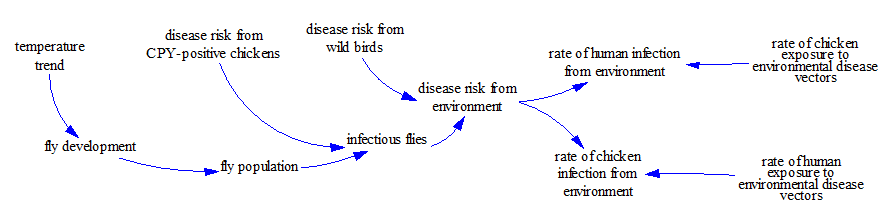
\includegraphics[width=0.5\textwidth]{images/environmental_submodel2.png}
	\caption{Diagram of the environmental sub-model}
	\label{fig:environmental_submodel}
\end{figure*}

\textit{Campylobacter} need humid surfaces to live, so surface water is recognised as a key player. Since animal faeces and runoff from agriculture and slaughterhouses enter nearby bodies of water, it is considered a good indicator for the amount of \textit{Campylobacter} present in the environment. Therefore, this has a big role in determining the chance of infection by biological disease vectors mentioned before. This can be seen in Figure~\ref{fig:environmental_submodel}. The main biological disease vectors have been determined to be flies and wild birds \parencite{mughini-gras_quantifying_2016}. Both vectors are considered to be major spreaders as they actively excrete \textit{Campylobacter} on surfaces and human food \parencite{french_molecular_2009, hald_influxed_2008, berndtson_campylobacter_1996}.

It seems that the vector potential of flies is mainly determined by the \textit{Brachycera} suborder of the order \textit{Diptera}, and to be more specific by the \textit{Musca domestica}, which is more commonly known as the house fly \parencite{hald_influxed_2008}. We therefore opt to use the \textit{Musca domestica} as the model organism to represent the effects of the \textit{Diptera} insect order. \cite{skovgard_retention_2011} suggests that \textit{Musca domestica} are mainly short distance carriers of \textit{Campylobacter}. Therefore, the risk of transmission by \textit{Musca deomstica} is particularly high when the populations are greatest, which is during summer \parencite{royden_role_2016}. \cite{hald_use_2007} showed that preventing flies from entering houses in the summer of 2006 caused a significant drop in the prevalence of \textit{Campylobacter} at farms.

In Dutch and Luxembourgish waters, 37.7\% and 61.0\% of the \textit{Campylobacter} strains were attributed to poultry and wild birds respectively in a research by \cite{mughini-gras_quantifying_2016}. Since Luxembourg has a low poultry production, it is important to include this biological transmission vector in the sub-model.

Extreme temperatures are important selective agents during the separate stages of the \textit{Brachycera}. Climate change will cause the number of \textit{Brachycera} in the Netherlands to increase \parencite{goulson_predicting_2005}. It is expected this rise in numbers will be most evident in summer, but it is also expected in the winter according to \citeauthor{goulson_predicting_2005}. The climate driven population growth will also trigger migration, and therefore the dispersal \parencite{feder_locomotion_2010}, which will result in increased transmission of \textit{Campylobacter}. It is suspected that the total number of birds in the Netherlands is not affected by climate change, just their composition \parencite{mclean_reduced_2020, knudsen_challenging_2011}. Rainfall is not a driving factor in the total \textit{Brachycera} biomass \parencite{goulson_predicting_2005}.

Climate change is also linked to different precipitation patterns in the Netherlands. An increase in precipitation will result in increase of the Dutch sewer systems being overwhelmed and dumping the overflow in the environment, and will also result in an increase of contaminated runoff from agriculture and slaughterhouses \parencite{kwaad_summer_1991}.

An increase in Dutch population size is not expected to increase the \textit{Brachycera} biomass in the Netherlands \parencite{guenat_effects_2019}. Even though an increase in the population leads to more organic waste \parencite{garcia-garcia_framework_2015}, which does have the potential to increase the total number of flies \parencite{imai_population_1984, rozendaal_houseflies_1997}, this effect is possibly counterbalanced by the loss of natural habitat.

%Effect of climate change on runoff of Campylobacter and Cryptosporidium from land to surface water  This study shows that for the evaluated scenarios, climate change has little impact on concentrations of Campylobacter and Cryptosporidium transported from land to the surface waters.

% Seasonal effect on probability of infection through surface water?


\subsubsection*{Infected chickens}
% add sub-model diagram here
The CLD presented in Figure \ref{fig:transmission_submodel} is a simplification of Rommens' 2020 model of dynamics of transmission  and contamination in farms, broilers and slaughterhouses \parencite{rommens_infected_2020}. Healthy chickens become infected with \textit{Campylobacter} due to environmental disease vectors such as flies \parencite{royden_role_2016}, that themselves can become infected from chicken \parencite{skovgard_retention_2011}. These infected chickens then can become contaminated chicken meat when slaughtered, and they can also cause cross-contamination, making the meat of healthy chicken also potentially contaminated when it enters into contact with the bacteria \parencite{berndtson_campylobacter_1996}. Contaminated meat is consumed and that will have a chance of infecting humans \parencite{wilson_tracing_2008}.

This section of the model behaves as the "success to the successful" archetype \parencite{pruyt_triple_2013}, where the feedback loops around the rate of chicken infection imply that when there are low infections, it is prone to stay that way, but when infections rise, it is difficult to limit their growth. The implications for our model is that a small push in the direction of infections can have big implications.

\begin{figure}[h]
\centering
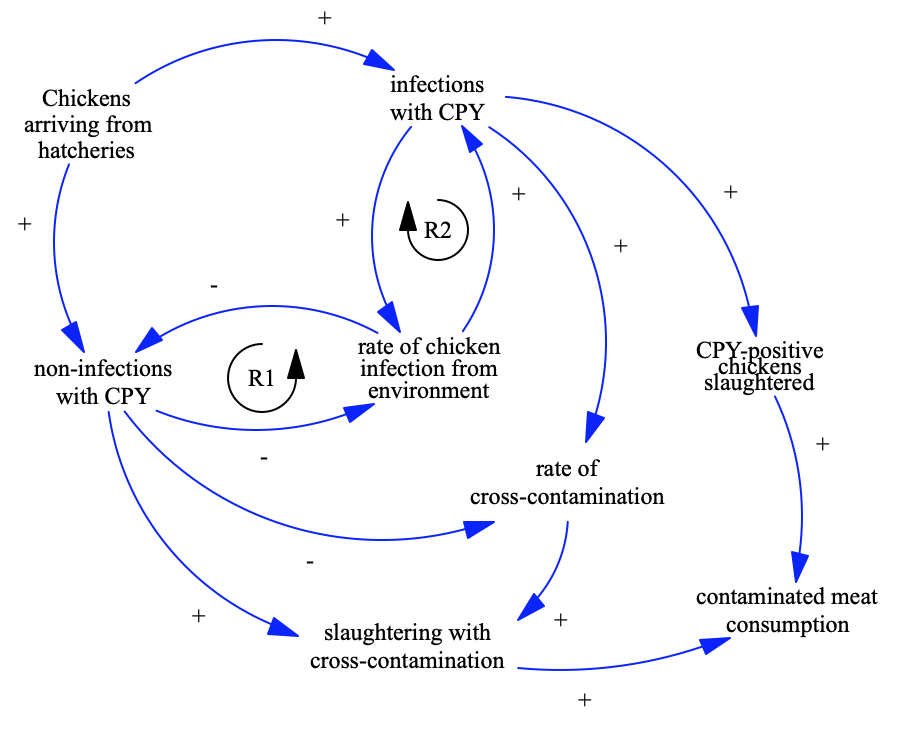
\includegraphics[width=1\textwidth]{images/Transmission submodel.png}
\caption{Conceptual causal loop diagram for chicken infection and contamination}
\label{fig:transmission_submodel}
\end{figure}

Other internal variables in this model included probabilities of infection, which are determined by environmental factors such as concentration of \textit{Campylobacter} in surface water, propagation of disease vectors, and climate effects, with the exact values for these rates detailed in Appendix~\ref{ch:model_documentation}.


\subsubsection*{Cost of illness}
%Emily
\begin{figure}[h]
\centering
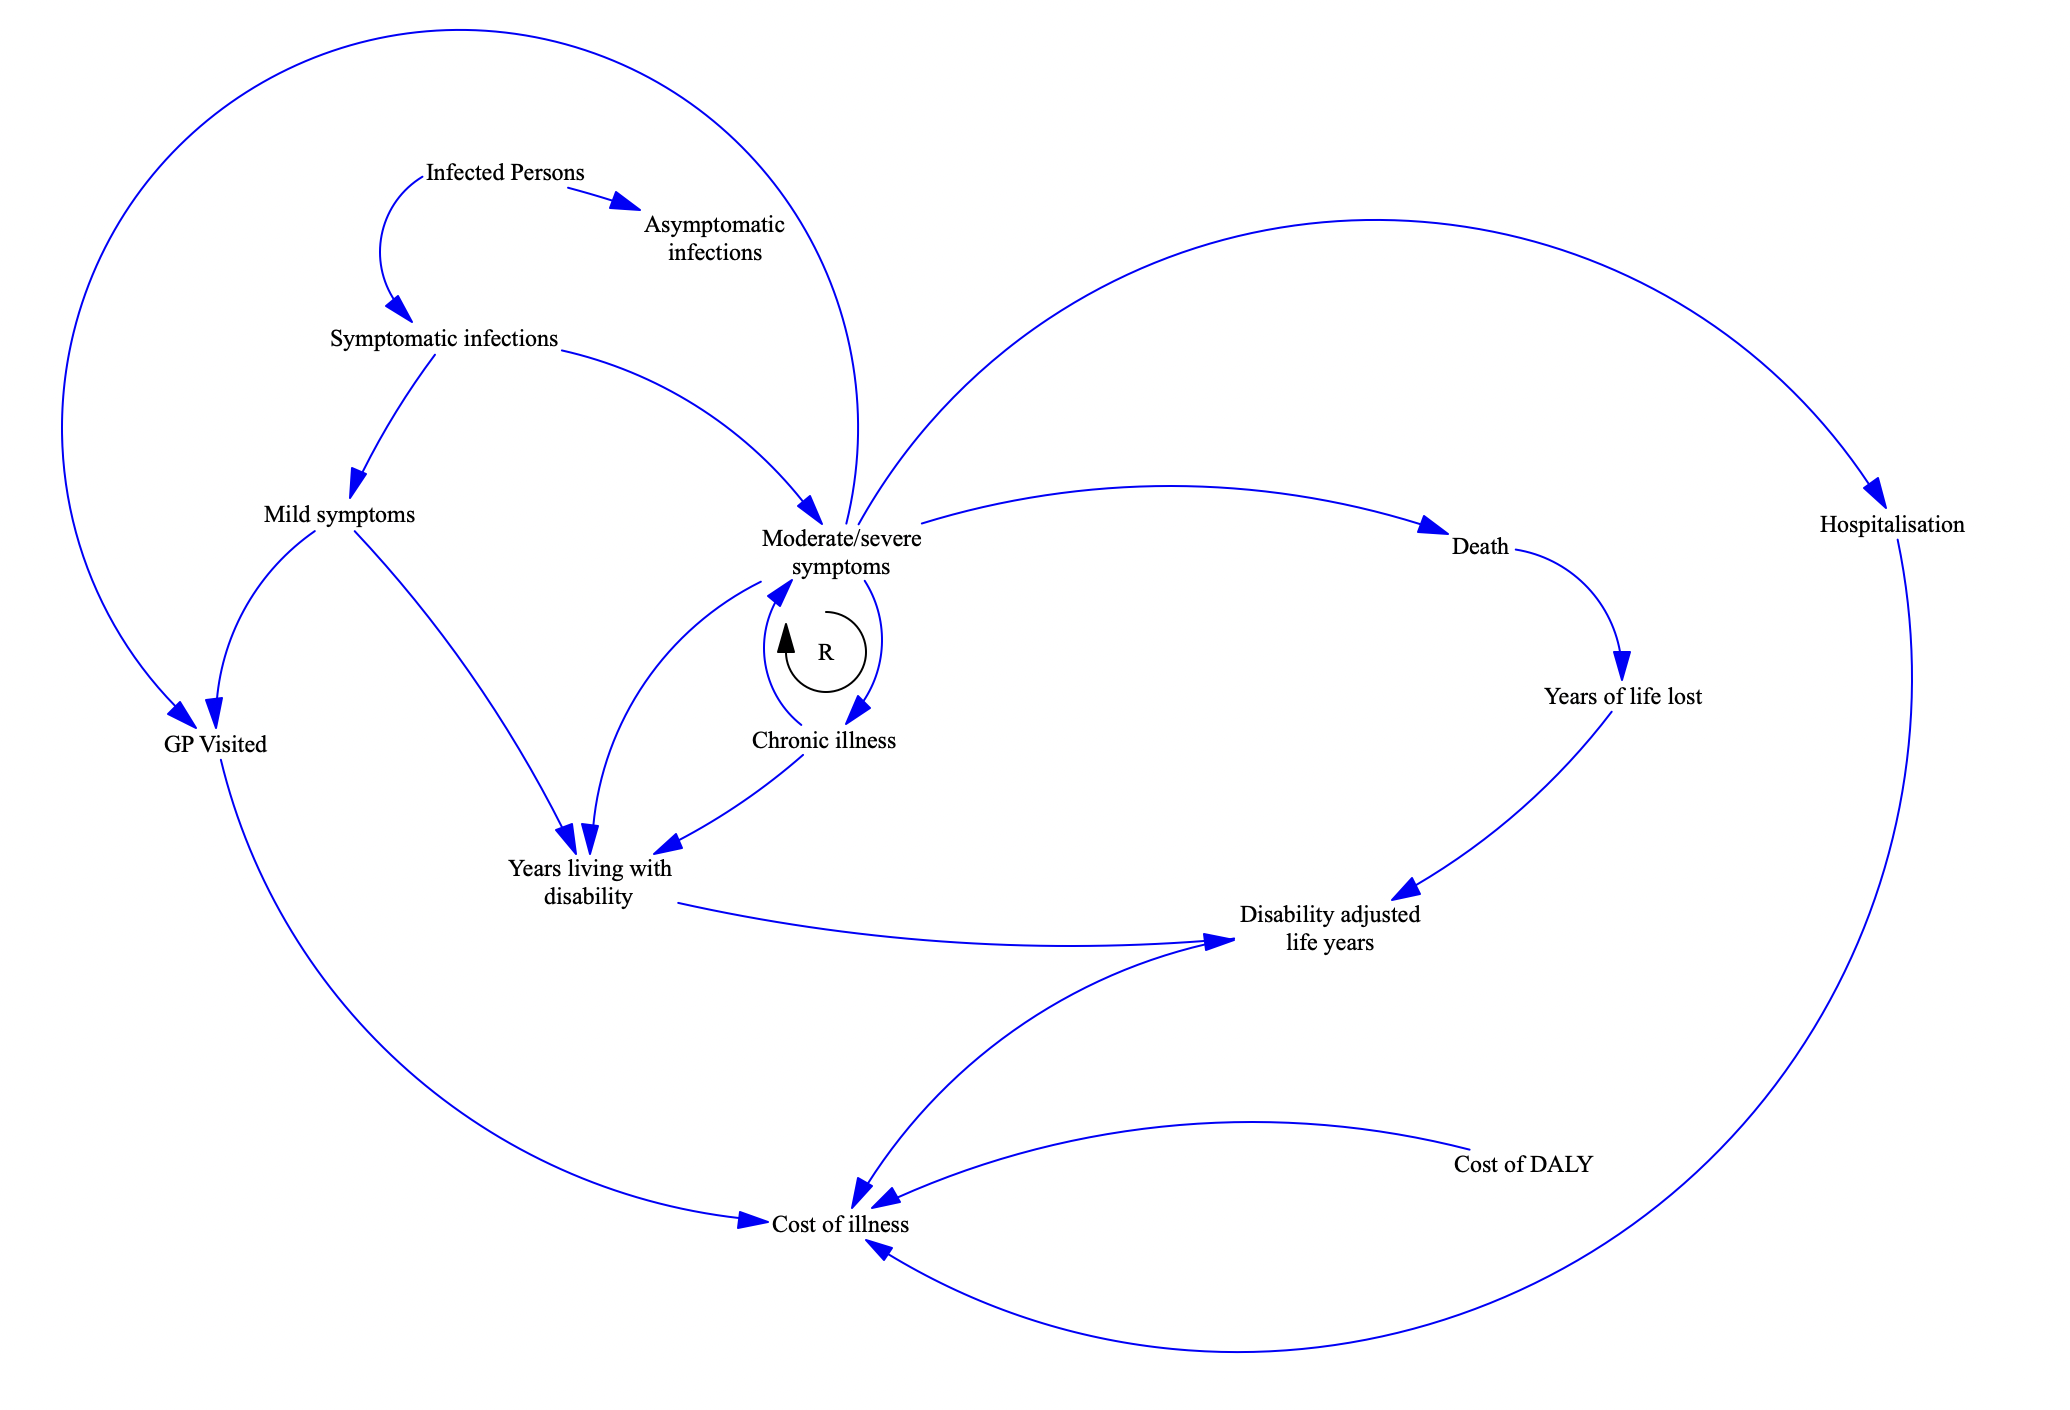
\includegraphics[width=\textwidth]{images/COI_submodel.png}
\caption{The conceptual Cost of Illness sub-model}
\end{figure}
The cost of illness associated with \textit{Campylobacter} infections was modelled and calculated based primarily on a 2007 study by Mangen \parencite{mangen_campylobacteriosis_2007}. The Infected Persons stock is split off into symptomatic and asymptomatic infections. Symptomatic infections are assumed to all develop acute gastroenteritis, with a proportion of all cases either recovering, or subsequently developing chronic illnesses. Each of these outcomes contribute to key public health metrics of Disability Adjusted Life Years (DALYs) for these infections, and the Cost of Illness for all \textit{Campylobacter} infections. 

The causal structure adopted for this sub-model focuses on connecting variables based on available scientific data. Due to the underlying complexity of DALY and Cost of Illness metrics \parencite{jo_cost--illness_2014}, a top-down approach to applying these variables has been taken. As such, variables have been used for some elements that might otherwise have been modelled as stocks (e.g. DALYs and Cost of Illness). Additionally, this more simplistic approach is considered appropriate, as we are not concerned with the detailed dynamics of transmission and recovery (as might be done in an SIR model), but only with the ultimate KPIs of 'DALY' and 'Cost of Illness'.

\subsection{Key Assumptions}
%What were the key assumptions made in developing the model?
    %Take from validation spreadsheet
    %Include simplifications of real-world circumstances (e.g. acute campy coming before chronic conditions)
\subsubsection{Assumptions}
The main assumptions made in modelling these causal structures are:
\begin{itemize}
    \item Demand for chicken meat exactly matches supply of chicken meat
    \item All chicken meat consumed in the Netherlands is produced in the Netherlands
    \item The disease burden and cost of illness associated with death from gastroenteritis is accounted for within the DALY and Cost of Illness values used.
    \item The development of chronic disease is assumed to always occur subsequent to a case of acute gastroenteritis (in reality, some cases will develop chronic disease without first developing gastronenteritis, following a \textbf{Campylobacter} infection.
\end{itemize}

Multiple assumptions on the values of individual parameters have been made, due to the absence of adequate literature. Where this is the case, the assumption has been noted in \textcolor{red}{table x in appendix y}.
\subsubsection{Simplifications}

\subsection{Model Specification}
%What are the main mechanisms/variables/parameters in our model?
\subsubsection{Mechanisms employed}
The main mechanisms employed in each part of the model are as follows:
\begin{itemize}
    \item Chicken infections: the chicken infections part of the model focuses on stock-flow structures to model accumulation and delays in the infection of chickens.
    \item Cost of illness: the cost of illness model relies on accumulation over time, while using a pulse-train mechanism to 'empty' the annual occurrence of acute illness.
    \item Environmental transmission: this part of the model replicates empirical models of insect development cycles, and translates this to prevalence of environmental transmission of \textit{Campylobacter} by disease vectors.
\end{itemize}

A full and detailed list of variables and parameters used in the model are detailed in \textcolor{red}{APPENDIX}.
%What software was used for the modelling?
\subsubsection{Modelling software used}
The system was modelled using VenSim PLE software developed by Ventana Systems Inc.
%Model Settings
    %Why was the integration method chosen?
    
\subsubsection{Integration method}
The model uses Euler as the integration method. Euler was considered an attractive integration method for this model as it is suitable for integrating over non-linear and discontinuous functions (such as the pulse trains used to drain stocks), and it is a simple a direct method of integration. However, it does present some limitations in computational inefficiencies.

\subsubsection{Time step}
    %Why was the time step chosen?
The time step of \textcolor{red}{X} was selected as behaviour of the model was consistent for this time step, and for half this time step. This suggests that the time steps are small enough such that the derivative of the model is constant between two very close points in time.
\textcolor{red}{Consider adding screenshot to show difference between two step sizes}

\textcolor{red}{Results presented start at Week X to allow for effects of delays and time constants to settle}

\subsubsection{Time period}
    %Why was the time period chosen
The time period of \textcolor{red}{X} years was chosen to be able to show the effects of incremental changes in climate variability, whilst maintaining a small enough time step such that the transmission within chicken farms is realistic.

\textcolor{red}{David: probs about 30 years (until 2050), else it is difficult to see any change from climate change, verify this with group on Friday.}

\subsection{Model Verification and Validation}
%4.	Validation
 %   a.	Use various tests to argue why model is fit for purpose
In this subsection we'll verify and validate the model. Verification will be done through a comparison with the conceptualisation of the model, as well as a unit verification and a time step verification. 

\subsubsection{Verification}

% From meeting with Jill:
%Verification requires three steps:
    %Check that the causal diagrams match the stock-flow diagrams, and add one line saying "this was checked'
    
To verify the conceptualisation, it was checked that the causal diagram construed in chapter \ref{s:conceptualisation} matches the model built. There have been some addedums to the model, but the functions still match.  
    %Check that the units are consistent with the real world and add one line saying 'units were checked for material consistency'. -- DONE
Unit verification was performed by checking all variable units for ensure consistency with real-world equivalents. There was one anomalous variable in the model which could not be mapped to a physical value. This refers to the \textit{balancing constant} that feeds into the \textit{rate of fly development}. This was added under the assumption that temperature linearly correlates to fly populations, as documented by \citeauthor{blanckenhorn_adaptive_1998}, 1998. This factor allows conversion from the units of temperature (degrees) to fly development rate (MFly per week). This cannot be done without adding a go-between, which, in our case, is the balancing constant. 

Another noteworthy unit is that of the flow of \textit{Symptomatic infections}. The time unit used in the model is \textit{week}, to properly integrate seasonal changes in temperature across the year, months being to big and days too detailed. But for this same reason, DALY and COI are commonly reported per year. To deal with this, a PULSE TRAIN function was installed between stocks \textit{CPY Cases} and \textit{Acute GE Cases}. The PULSE TRAIN accumulates all \textit{Campylobacteriosis} cases over 52 weeks before transferring them to the cost of illness submodel. This can then be used as an input per year for the COI submodel. The units of the PULSE train remain in weeks when the time unit should be thought of as year, as happens after. 
    %Confirm that you've used the appropriate numerical technique/time step and add one line saying, 'behaviour of the model for the chosen time step and half that time step is consistent, this indicates that the appropriate time step and integration method has been used'
    
The time step verification was performed by running the model at several different time steps. The time step \textcolor{red}{X} is chosen so the integration method (Euler) is valid. When halving the time step, we found that model returned similar model behaviour, with the exception of one flow, the \textit{symptomatic infections}. This is because this flow uses a PULSE TRAIN, as described above and this pulse train depends on the time step. Because of this, when the time step is halved, the PULSE TRAIN becomes far bigger. However, this has no effect on the stock it goes into, the number of acute cases 

% WHY???? 

    
\subsubsection{Validation}    

%Validation requires three steps:
    %Show how the data matches or does not match historical data (explain why)
    
\textcite{vlaanderen_staat_2019} estimated there were around 71.000 cases of Campylobacteriosis in the Netherlands in 2018, 67.000 in 2017 and 79.000 in 2016. We plotted the amount of cases produced by our model against the average of these three values. The results can be seen in Figure~\ref{fig:val_human_cases} Our model never exceeds that number, since it is a simplified version of reality, and certain disease vectors have been left out.

\textcite{nepluvi_rapportage_2019} monstered broiler chickens weekly in 2018, and found $41,9$-$58.1\%$ of broilerchickens were tested positive for \textit{Campylobacter}. This concerns chickens from slaughterhouses. As can be seen in Figure~\ref{fig:val_chickens}, in our model this number is an order of magnitude lower. NEED TO GIVE REASON

In the Netherlands the (unsanitary) preparation and / or consumption of chicken were attributed to $20$-$30\%$ of infections in 2018. However, around $50$-$80\%$ of cases can be attributed to \textit{Campylobacter} strains associated with poultry \parencite{cuperus_surveillance_2020, nepluvi_rapportage_2019}. Therefore, it is safe to assume that there are multiple transmission routes. We assume this transmission route can be found in the environment, and because of these facts, we assume the environmental transmission routes play a bigger role. Around $20$-$60\%$ of the human infections are from the environment. As can be seen in Figure~\ref{fig:val_sources} this is not the case in our model. The majority of the infections stem from food consumption. NEED TO GIVE REASON

We also validated our DALYs and Cost of Illness against the datapoints from RIVM. We plotted them against the average of the values mentioned in \citetitle{vlaanderen_staat_2019}, 
\textbf{DALYs} \\
\parencite{vlaanderen_staat_2019} \\
2016 2017 2018 \\
3.573 3.074 3.201

% diagnosis of chronic diseases attributed to CBD has increased in the past years
% whole numbers lol

\textbf{CoI} \\
\parencite{vlaanderen_staat_2019} \\
64 55 64 M\euro{} \\


\textbf{flies} \\
It is estimated there are around 17 million species of \textit{Diptera} per person \parencite{gorman_trillions_2017}. We are only interested in \textit{Musca domestica}. It is unknown what their numbers are in the Netherlands, and we are unable to estimate. However, it has been guessed that the population of Houseflies will increase by 244\% by 2080 \parencite{mcalister_secret_2017}.

\iffalse
\textbf{Extra}\\
\textcite{vlaanderen_staat_2019} and curperus also show the actual human infections confirmed by laboratoria from 2006-2018, and the numbers for the Netherlands. I assumed these were uninteresting, since we also care about untested individuals

The use of antacids may increase one's chances of getting Campylobacteriosis. This is structural uncertainty we could include.

\textcite{vlaanderen_staat_2019} shows that campylobacter is becoming resistant against antibiotics: also uncertainty.


I suppose the factor wild birds play can also be considered uncertain. There are still a lot of gaps in the literature regarding disease transmission amongst birds and from birds to other animal taxa.
\fi

    %Conduct an extreme values test to test the dynamic hypothesis and range of model applicability and provide comment to the reader on the boundaries of the model's effective use. Tell the reader the conditions under which the model behaves reliably
    
    
    %Generate the mode of behaviour/dynamic hypothesis - does it match, why or why not?
    
\subsection{Experimental setup}
%5.	Experimental setup
 %   a.	Introduce main uncertainties (potentially with table)
  %  b.	Explain scenario and policy logic
  
        %Parametric experiments - change parameters and observe behaviour (do multivariate for all, and univariate for one or two key variables)
        %Structural experiments - change a structure (e.g. add feedback) and observe behaviour 
   % c.	Number of runs, numerical integration method & time step, versions, etc.: all justified

%Policies in environment
\subsubsection{Environmental factors and policies to control disease vectors}
\begin{itemize}
    \item Public campaigns to prevent human exposure to infected flies: on the season when the disease vector is more prevalent, urge the population to keep organic waste properly closed and use fly nets \parencite{hald_use_2007}. Similar measures are used to prevent the reproduction of disease carrying mosquitoes in tropical countries. %I know this for a fact because tropical country, but we might want to add a source.
    \item Pest control measures: when a certain threshold of fly population is reached, the government can initiate extermination campaigns to limit the spread of diseases. This can be generalized, or localized only around farms.
%install pest control measures, including variables such as: intensity of extermination / frequency
%install threshold fly population value that activates pest control. The aim is to counteract effects of population growth to infected flies and infection rates.
%Note: could we connect fly population or proportion of infected flies to exposure rate??
\end{itemize}

\subsubsection{Chicken production and policies}
%Policies on chicken farms
\begin{itemize}
    \item Improve sanitation of slaughterhouse equipment: requirement for slaughterhouse equipment to be cleaned using water that is frequently changed to prevent cross-contamination. Additionally, this can be accompanied by the use of UV radiation to aid in the decontamination process without altering the sensory quality of the meat \parencite{isohanni_use_2009}.
    \item Logistic slaughter: process infected chicken last to prevent cross-contamination of chicken meat. Requires testing for infection in farms and it is possible for undetected infected chickens to go first \parencite{evers_predicted_2004}. 
\end{itemize}

\subsubsection{Food safety behaviours and policies}

%Policies in COI 
\begin{itemize}
    \item Food safety and handling: Policy connecting cost of illness to proportion of contaminated chicken
    \item Behavioural link from DALYs to either infections per kg consumed OR kg of chicken meat consumed. There is a structural uncertainty related to how consumer behaviour might change. Will individuals reduce their chicken consumption or will they be more careful in food handling?
    % 
    \item 
\end{itemize}